%%%
% Plantilla de Memoria
% Modificación de una plantilla de Latex de Nicolas Diaz para adaptarla 
% al castellano y a las necesidades de escribir informática y matemáticas.
%
% Editada por: Mario Román
%
% License:
% CC BY-NC-SA 3.0 (http://creativecommons.org/licenses/by-nc-sa/3.0/)
%%%

%%%%%%%%%%%%%%%%%%%%%%%%%%%%%%%%%%%%%%%%%
% Thin Sectioned Essay
% LaTeX Template
% Version 1.0 (3/8/13)
%
% This template has been downloaded from:
% http://www.LaTeXTemplates.com
%
% Original Author:
% Nicolas Diaz (nsdiaz@uc.cl) with extensive modifications by:
% Vel (vel@latextemplates.com)
%
% License:
% CC BY-NC-SA 3.0 (http://creativecommons.org/licenses/by-nc-sa/3.0/)
%
%%%%%%%%%%%%%%%%%%%%%%%%%%%%%%%%%%%%%%%%%

%----------------------------------------------------------------------------------------
%	PAQUETES Y CONFIGURACIÓN DEL DOCUMENTO
%----------------------------------------------------------------------------------------
%%% Configuración del papel.
% microtype: Tipografía.
% mathpazo: Usa la fuente Palatino.
\documentclass[a4paper, 11pt]{article}
\usepackage[protrusion=true,expansion=true]{microtype}
\usepackage{mathpazo}


% Indentación de párrafos para Palatino
\setlength{\parindent}{0pt}
  \parskip=8pt
\linespread{1.05} % Change line spacing here, Palatino benefits from a slight increase by default


%%% Castellano.
% noquoting: Permite uso de comillas no españolas.
% lcroman: Permite la enumeración con numerales romanos en minúscula.
% fontenc: Usa la fuente completa para que pueda copiarse correctamente del pdf.
\usepackage[spanish,es-noquoting,es-lcroman]{babel}
\usepackage[utf8]{inputenc}
\usepackage[T1]{fontenc}
\selectlanguage{spanish}


%%% Gráficos
\usepackage{graphicx} % Required for including pictures
\usepackage{wrapfig} % Allows in-line images
\usepackage[usenames,dvipsnames]{color} % Coloring code

%%% Matemáticas
\usepackage{amsmath}


%%% Bibliografía
\makeatletter
\renewcommand\@biblabel[1]{\textbf{#1.}} % Change the square brackets for each bibliography item from '[1]' to '1.'
\renewcommand{\@listI}{\itemsep=0pt} % Reduce the space between items in the itemize and enumerate environments and the bibliography
\usepackage{hyperref}
\hypersetup{
	colorlinks   = true,    % Colours links instead of ugly boxes
	urlcolor     = red,    % Colour for external hyperlinks
	linkcolor    = red,    % Colour of internal links
	citecolor    = blue      % Colour of citations
}
%%% CÓDIGO
\usepackage{listings}
\usepackage{courier}
\lstset{
	basicstyle=\footnotesize\ttfamily, % Standardschrift
	numbers=left,               % Ort der Zeilennummern
	numberstyle=\tiny,          % Stil der Zeilennummern
	stepnumber=1,               % Abstand zwischen den Zeilennummern
	numbersep=5pt,              % Abstand der Nummern zum Text
	tabsize=2,                  % Groesse von Tabs
	extendedchars=true,         %
	breaklines=true,            % Zeilen werden Umgebrochen
	keywordstyle=\color{red},
	frame=b,         
	%        keywordstyle=[1]\textbf,    % Stil der Keywords
	%        keywordstyle=[2]\textbf,    %
	%        keywordstyle=[3]\textbf,    %
	%        keywordstyle=[4]\textbf,   \sqrt{\sqrt{}} %
	stringstyle=\color{white}\ttfamily, % Farbe der String
	showspaces=false,           % Leerzeichen anzeigen ?
	showtabs=false,             % Tabs anzeigen ?
	xleftmargin=17pt,
	framexleftmargin=17pt,
	framexrightmargin=5pt,
	framexbottommargin=4pt,
	%backgroundcolor=\color{lightgray}
	showstringspaces=false      % Leerzeichen in Strings anzeigen ?        
	literate=
	{á}{{\'a}}1 {é}{{\'e}}1 {í}{{\'i}}1 {ó}{{\'o}}1 {ú}{{\'u}}1
	{Á}{{\'A}}1 {É}{{\'E}}1 {Í}{{\'I}}1 {Ó}{{\'O}}1 {Ú}{{\'U}}1
	{à}{{\`a}}1 {è}{{\`e}}1 {ì}{{\`i}}1 {ò}{{\`o}}1 {ù}{{\`u}}1
	{À}{{\`A}}1 {È}{{\'E}}1 {Ì}{{\`I}}1 {Ò}{{\`O}}1 {Ù}{{\`U}}1
	{ä}{{\"a}}1 {ë}{{\"e}}1 {ï}{{\"i}}1 {ö}{{\"o}}1 {ü}{{\"u}}1
	{Ä}{{\"A}}1 {Ë}{{\"E}}1 {Ï}{{\"I}}1 {Ö}{{\"O}}1 {Ü}{{\"U}}1
	{â}{{\^a}}1 {ê}{{\^e}}1 {î}{{\^i}}1 {ô}{{\^o}}1 {û}{{\^u}}1
	{Â}{{\^A}}1 {Ê}{{\^E}}1 {Î}{{\^I}}1 {Ô}{{\^O}}1 {Û}{{\^U}}1
	{œ}{{\oe}}1 {Œ}{{\OE}}1 {æ}{{\ae}}1 {Æ}{{\AE}}1 {ß}{{\ss}}1
	{ű}{{\H{u}}}1 {Ű}{{\H{U}}}1 {ő}{{\H{o}}}1 {Ő}{{\H{O}}}1
	{ç}{{\c c}}1 {Ç}{{\c C}}1 {ø}{{\o}}1 {å}{{\r a}}1 {Å}{{\r A}}1
	{€}{{\euro}}1 {£}{{\pounds}}1 {«}{{\guillemotleft}}1
	{»}{{\guillemotright}}1 {ñ}{{\~n}}1 {Ñ}{{\~N}}1 {¿}{{?`}}1   
}


\lstloadlanguages{% Check Dokumentation for further languages ...
	%[Visual]Basic
	%Pascal
	%C
	C++
	%%XML
	%%HTML
	%Java
}
%\DeclareCaptionFont{blue}{\color{blue}} 

%\captionsetup[lstlisting]{singlelinecheck=false, labelfont={blue}, textfont={blue}}
\usepackage{caption}
\DeclareCaptionFont{white}{\color{white}}
\DeclareCaptionFormat{listing}{\colorbox[cmyk]{0.43, 0.35, 0.35,0.01}{\parbox{\textwidth}{\hspace{15pt}#1#2#3}}}
\captionsetup[lstlisting]{format=listing,labelfont=white,textfont=white, singlelinecheck=false, margin=0pt, font={bf,footnotesize}
}

%% cosas 

\usepackage[margin=1in]{geometry}

\usepackage{times}








%----------------------------------------------------------------------------------------
%	DOCUMENTO
%----------------------------------------------------------------------------------------

\begin{document}
	
	
	\begin{titlepage}
		\begin{center}
			\vspace*{2cm}
			
			{\Huge \textbf Cuaderno de prácticas FBD.}
			
			
			\vspace{0.5cm}
			
			
		    \centering \includegraphics[width=0.9\textwidth]{cover.jpg}
		    
			
			\vspace{2cm}
			
			\textbf{Francisco Navarro Morales - GRG121 }
			
			\vfill
			
			Segundo curso del Grado de Ingeniería Informática\\
			Universidad de Granada\\
			curso 2016-2017\\
			
		\end{center}
	\end{titlepage}


%\maketitle % Print the title section

%% Resumen (Descomentar para usarlo)
\renewcommand{\abstractname}{Resumen} % Uncomment to change the name of the abstract to something else
%\begin{abstract}
% Resumen aquí
%\end{abstract}

%% Palabras clave
%\hspace*{3,6mm}\textit{Keywords:} lorem , ipsum , dolor , sit amet , lectus % Keywords
%\vspace{30pt} % Some vertical space between the abstract and first section


%% Índice
{\parskip=2pt
  \tableofcontents
}

%%% Inicio del documento

\pagebreak

\section{Punto 2. Creación de la BD}
\subsection{ Ejercicio 2.6: Modifica el esquema de la tabla plantilla añadiendo un nuevo atributo llamado fechabaja de tipo date.}	
ALTER TABLE ADD DATE FECHABAJA
\subsection{ Ejercicio 2.8: Ejecuta la sentencia SELECT para mostrar el contenido de las tablas PRUEBA2 y PLANTILLA. Intenta mostrar sólo algunos campos de las mismas.}
select cad, dni from prueba2, plantilla	
\subsection{Ejercicio 2.9 Ejecuta la sentencia UPDATE sobre la tabla plantilla y cambia el nombre del trabajador con dni ’12345678’ a ’Luis’.}
update table plantilla 
	set nombre = 'Luis' where dni = '12345678';
	
\subsection{Ejercicio 2.10 Borra todas las tuplas de la tabla plantilla.
	SQL> DELETE FROM plantilla;
	En este caso da un mensaje de error (¿por qué?). Aunque sí podríamos borrar las tuplas
	de la tabla serjefe.
	SQL> DELETE FROM serjefe;}
Se debe a que la tabla plantilla es referenciada por un atributo de la tabla serjefe y no puede ser borrada sin modificar antes esta circunstancia o borrar la tabla serjefe. Si borramos la tabla serjefe y, a continuación, borramos la tabla plantilla, no dará problemas.


\subsection{Ejercicio 2.11 A continuación vamos a tratar de insertar algunas tuplas nuevas en ventas.
	Comprueba que se introducen correctamente y, en caso contrario, razona por qué da error.}
\begin{itemize}
	\item  $insert\ into\ ventas\ values\ (’S3’, ’P1’, ’J1’, 150, ’24/12/05’);$
	Da error porque el valor de la fecha no se está entendiendo como una fecha, hay que utilizar la directiva `TO\_DATE' de la forma:
	$insert\ into\ ventas\ values\ ('S3', 'P1', 'J1', 150, TO\_DATE('24/12/05','dd/mm/yyyy'));$
	\item $insert\ into\ ventas\ (codpro, codpj)\ values\ (’S4’, ’J2’);$  el error lo provoca no insertar ningún valor para el campo codpie, que tiene una restricción de $not\ null$ que impide que no se le asigne ningún valor. 
	\item $insert\ into\ ventas\ values(’S5’,’P3’,’J6’,400,TO_DATE(’25/12/00’));$ falla porque la sentencia $TO\_DATE$ está incompleta, ya que le falta el formato. Para que fuera correcta debería tener: $TO\_DATE('25/12/00','dd/mm/yyyy')$
\end{itemize}
	
\subsection{Ejercicio 2.12 Actualizar la fecha del proveedor S5 al año 2005’}
No hay que hacer nada, funciona perfectamente.
$UPDATE\ ventas\
SET\ fecha\ =\ TO\_DATE(2005,’YYYY’)
WHERE codpro=’S5’;$

\subsection{Ejercicio 2.13 Para mostrar la columna FECHA con un formato específico e imprimirla, utilizar la siguiente sentencia:}
$select\ codpro,codpie,\ to_char(fecha,’"Dia" day,dd/mm/yy’)\ from ventas;$ funciona correctamente.

\subsection{Ejercicio 2.14 Dado el esquema siguiente de la base de datos de una liga de baloncesto:}
  \centering 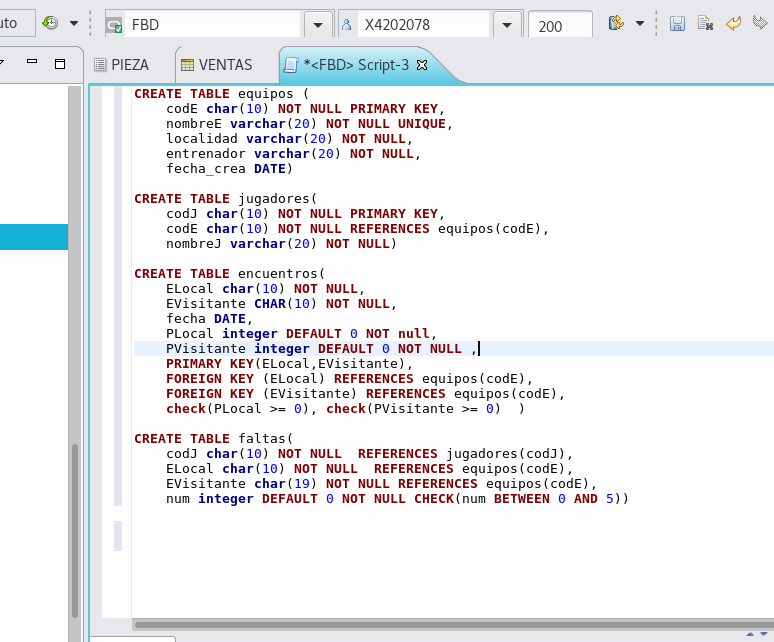
\includegraphics[width=0.9\textwidth]{1.png}
\subsection{Ejercicio 2.15 Preparar un archivo para la introducción de datos en las tablas Equipos,
	Jugadores, Encuentros y Faltas, conforme a los siguientes criterios, para que nos permitan
	realizar consultas con resultados significativos.
	Que se inserten 4 equipos con 5 jugadores en cada uno.
	Que se inserten 10 encuentros (no se ha terminado la liga).
	Que se inserten los resultados esos encuentros dejando un único equipo invicto.}
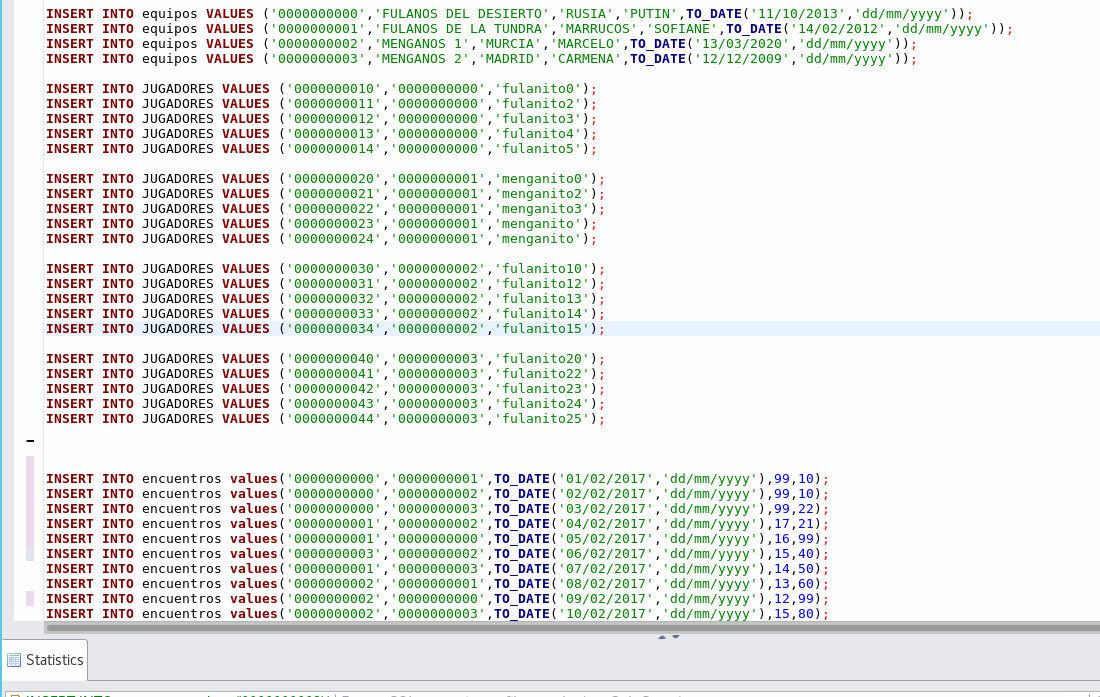
\includegraphics[width=0.9\textwidth]{2.png}

\section{Punto 3.  PRACTICA 2, CONSULTAS.}
\subsection{Ejercicio 3.1 Comprueba el resultado de la proyección. ¿Es éste conforme a lo que se obtiene
	en el AR?}
Se obtiene Londres,Londres,Paris,Roma, que es distinto de lo obtenido en AR porque AR no da resultados repetidos. Para evitar que se repitan resultados en SQL habría que utilizar select distinct 
\subsection{Ejercicio 3.2 Muestra los suministros realizados (tan solo los códigos de los componentes
	de una venta). ¿Es necesario utilizar DISTINCT?}
No hace falta poner unique porque uno de los atributos mostrados es clave primaria y por tanto no va a haber ninguna tupla repetida.

\subsection{Ejercicio 3.3 Muestra las piezas de Madrid que son grises o rojas.}
$SELECT\ *\ FROM\ pieza\ WHERE\ color\ IN\ ('Rojo','Gris')\ AND\ ciudad\ =\ 'Madrid'$

P1 	Tuerca	Gris	2.5	Madrid

\subsection{Ejercicio 3.4 Encontrar todos los suministros cuya cantidad está entre 200 y 300, ambos
	inclusive.}
SELECT * FROM ventas WHERE CANTIDAD BETWEEN 200 AND 300

\subsection{Ejercicio 3.5 Mostrar las piezas que contengan la palabra tornillo con la t en
	mayúscula o en minúscula.}
SELECT codpie FROM PIEZA WHERE nompie IN ('Tornillo', 'tornillo')

\subsection{ Ejercicio 3.6 Comprueba que no devuelve ninguna. Pero SI que hay!!!}
efectivamente, no devuelve ninguna. Se debe a que existe la tabla ventas pero tiene el nombre en mayúsculas. Si utilizamos: $$Select\ table_name\ from\ ALL\_TABLES\ where\ TABLE\_NAME\ like\ 'VENTAS';$$ sí que funciona.

\subsection{Ejercicio 3.7 Resolver la consulta del ejemplo 3.8 utilizando el operador $\cap$.}

la consulta: $\pi_{ciudad} ( \sigma_{status>2}(proveedor)) - \pi_{ciudad}(\sigma_{cod\_pie='P1'}(pieza))$

se puede escribir como: $\pi_{ciudad}(\sigma_{status>2}(proveedor) \cap (  \pi_{ciudad}(proveedor) - \pi_{ciudad}(\sigma_{cod\_pie='P1'}(pieza))$

\subsection{Ejercicio 3.8 Encontrar los códigos de aquellos proyectos a los que sólo abastece ’S1’.}
$SELECT\ codpj\ FROM\ proyecto\ MINUS\ SELECT\ codpj\ FROM\ ventas\ WHERE\ codpro\ !=\ 'S1'$

\subsection{Ejercicio 3.9 Mostrar todas las ciudades de la base de datos. Utilizar UNION}
$SELECT\ ciudad\ FROM\ PIEZA\ UNION\ SELECT\ ciudad\ FROM\ PROVEEDOR\ UNION\ SELECT\ ciudad\ FROM\ proyecto $

\subsection{Ejercicio 3.10 Mostrar todas las ciudades de la base de datos. Utilizar UNION ALL}
$SELECT\ ciudad\ FROM\ PIEZA\ UNION\ ALL\ SELECT\ ciudad\ FROM\ PROVEEDOR\ UNION\ ALL\ SELECT\ ciudad\ FROM\ proyecto $

La única diferencia es que UNION no devuelve repetidos y UNION ALL sí.

\subsection{Ejercicio 3.11 Comprueba cuántas tuplas resultan del producto cartesiano aplicado a ventas
	y proveedor}

$SELECT\ count(*)\ FROM\ ventas,proveedor$

\subsection{Ejercicio 3.12 Mostrar las ternas que son de la misma ciudad pero que hayan realizado
	alguna venta.}
$SELECT\ *\ FROM\ pieza,ventas,PROVEEDOR,PROYECTO\ WHERE\ pieza.ciudad\ =\ proveedor.ciudad\ AND\ proveedor.ciudad\ =\ proyecto.ciudad\ AND\ ventas.CODPRO\ =\ proveedor.codpro\ AND\ ventas.codpie\ =\ pieza.codpie\ AND\ ventas.CODPJ\ =\ proyecto.codp$

\subsection{Ejercicio 3.13 Encontrar parejas de proveedores que no viven en la misma ciudad.}
$SELECT\ proveedor.CODPRO,\ pro.codpro\ FROM\ proveedor,\ proveedor\ pro\ WHERE\ proveedor.ciudad\ >\ pro.ciudad$

\subsection{Ejercicio 3.14 Encuentra las piezas con máximo peso.}

$
SELECT\ pieza.codpie\ FROM\ pieza\ MINUS\ SELECT\ pieza.codpie\ FROM\ pieza,\ pieza\ pie\ WHERE\ pieza.peso\ <\ pie.PESO$

\subsection{Ejercicio 3.15 Mostrar las piezas vendidas por los proveedores de Madrid.}


$SELECT\ DISTINCT\ codpie\ FROM\ ventas\ NATURAL\ JOIN\ proveedor\ WHERE\ proveedor.ciudad\ =\ 'Madrid'$

\subsection{Ejercicio 3.16 Encuentra la ciudad y los códigos de las piezas suministradas a cualquier
	proyecto por un proveedor que está en la misma ciudad donde está el proyecto.}
$
SELECT\ DISTINCT\ proveedor.ciudad,codpie\ FROM\ proveedor,\ proyecto,\ ventas\ WHERE\ proveedor.ciudad\ =\ proyecto.ciudad\ AND\ proveedor.codpro\ =\ ventas.codpro\ AND\ proyecto.codpj\ =\ ventas.codpj$

\subsection{Ejercicio 3.17 Comprobar la salida de la consulta anterior sin la cláusula ORDER BY.}
con order by: Jose Fernandez Luisa Gomez Manuel Vidal Maria Reyes Pedro Sanchez.

sin order by: Jose Fernandez
Manuel Vidal
Luisa Gomez
Pedro Sanchez
Maria Reyes.

\subsection{Ejercicio 3.18 Listar las ventas ordenadas por cantidad, si algunas ventas coinciden en la
	cantidad se ordenan en función de la fecha de manera descendente.}
SELECT\ *\ FROM \ ventas\ ORDER\ BY\ cantidad\ ASC,\ fecha\ DESC\ 


\subsection{Ejercicio 3.19 Mostrar las piezas vendidas por los proveedores de Madrid. (Fragmentando
	la consulta con ayuda del operador IN.) Compara la solución con la del ejercicio 3.15.}

$Select\ codpie
from\ ventas
where\ codpro\ IN
(select\ codpro\ from\ proveedor\ where\ ciudad\ =\ ’Londres’);$ 

Esta solución no requiere el natural join y se lee mejor que la del ejercicio 3.15:

$SELECT\ DISTINCT\ codpie\ FROM\ ventas\ NATURAL\ JOIN\ proveedor\ WHERE\ proveedor.ciudad\ =\ 'Madrid'$


\subsection{Ejercicio 3.20 Encuentra los proyectos que están en una ciudad donde se fabrica alguna
	pieza.}
$SELECT\ codpj\ FROM\ proyecto\ WHERE\ ciudad\ IN\ (SELECT\ ciudad\ FROM\ PIEZA)$

\subsection{Ejercicio 3.21 Encuentra los códigos de aquellos proyectos que no utilizan ninguna pieza
	roja que esté suministrada por un proveedor de Londres.}

$SELECT\ codpj\ FROM\ ventas\ MINUS\ SELECT\ codpj\ FROM\ ventas\ WHERE\ codpie\ IN\ (SELECT\ codpie\ FROM\ pieza\ NATURAL\ JOIN\ VENTAS\ WHERE\ color\ =\ 'Rojo'\ AND\ codpro\ IN\ (SELECT\ codpro\ FROM\ PROVEEDOR\ WHERE\ ciudad\ =\ 'Londres'))$

\subsection{Ejercicio 3.22 Muestra el código de las piezas cuyo peso es mayor que el peso de cualquier
	’tornillo’.}
$SELECT\ codpie\ FROM\ pieza\ WHERE\ NOT\ EXISTS\ (SELECT\ codpie\ FROM\ pieza\ pie\ WHERE\ pie.nompie\ =\ 'Tornillo'\ AND\ pie.peso\ >\ pieza.peso)$

\subsection{Ejercicio 3.23 Encuentra las piezas con peso máximo. Compara esta solución con la obtenida
	en el ejercicio 3.14}

$SELECT\ codpie\ FROM\ pieza\ WHERE\ NOT\ EXISTS\ (SELECT\ codpie\ FROM\ pieza\ pie\ WHERE\ pie.peso\ >\ pieza.peso)$

en el ejercicio 14: $SELECT\ pieza.codpie\ FROM\ pieza\ MINUS\ SELECT\ pieza.codpie\ FROM\ pieza,\ pieza\ pie\ WHERE\ pieza.peso\ <\ pie.PESO$

La principal diferencia es que al utilizar el minus restamos las piezas que pesan menos que alguna otra pieza (y quedan las que pesan mas que todas las demás) y al usar not exists seleccionamos aquellas piezas para las que no existe ninguna que pese más, es decir, se comprueba si existen piezas que pesen más. Luego la consulta es totalmente distinta.

\subsection{Ejercicio 3.24 Encontrar los códigos de las piezas suministradas a todos los proyectos
	localizados en Londres.}
$SELECT\ codpie\ FROM\ pieza\ WHERE\ NOT\ EXISTS\ (SELECT\ codpj\ FROM\ proyecto\ WHERE\ ciudad\ =\ 'Londres'\ AND\ NOT\ EXISTS\ (SELECT\ *\ FROM\ ventas\ WHERE\ pieza.codpie\ =\ ventas.codpie\ AND\ proyecto.codpj\ =\ ventas.codpj))$

\subsection{Ejercicio 3.25 Encontrar aquellos proveedores que envían piezas procedentes de todas las
	ciudades donde hay un proyecto.}$
SELECT\ codpro\ FROM\ proveedor\ WHERE\ NOT\ exists(
\ SELECT\ ciudad\ FROM\ pieza\ WHERE\ ciudad\ IN\ (SELECT\ DISTINCT\ ciudad\ FROM\ proyecto)\ AND\ NOT\ exists(
\ SELECT\ *\ FROM\ ventas\ WHERE\ proveedor.codpro\ =\ ventas.codpro\ AND\ pieza.codpie\ =\ ventas.codpie)
\ )
$





\end{document}